\begin{longtable}{r l p{10cm}}
	\midrule
	\multicolumn{2}{|c|}{Requisito} & Classi\tabularnewline
	\hline
	& \hyperlink{R-3V1}{R-3V1} & \hyperlink{client::controller::teacher::ManageQuestions}{client::controller::teacher::ManageQuestions}
	
	\hyperlink{client::view::teacher::ManageQuestions}{client::view::teacher::ManageQuestions}\tabularnewline
	\hline
	& \hyperlink{R-3F7}{R-3F7} & \hyperlink{client::controller::teacher::ManageQuestionnaires}{client::controller::teacher::ManageQuestionnaires}
	
	\hyperlink{client::controller::teacher::ManipulateQuestionnaire}{client::controller::teacher::ManipulateQuestionnaire}
	
	\hyperlink{client::model::data::CurrentQuestionnaire}{client::model::data::CurrentQuestionnaire}
	
	\hyperlink{client::model::data::CurrentQuestion}{client::model::data::CurrentQuestion}
	
	\hyperlink{client::model::service::QuestionnaireService}{client::model::service::QuestionnaireService}
	
	\hyperlink{client::view::teacher::ManageQuestionnaires}{client::view::teacher::ManageQuestionnaires}
	
	\hyperlink{client::view::teacher::ManipulateQuestionnaire}{client::view::teacher::ManipulateQuestionnaire}
	
	\hyperlink{server::app::App}{server::app::App}
	
	\hyperlink{server::data::Questionnaire}{server::data::Questionnaire}
	
	\hyperlink{server::service::QuestionnaireService}{server::service::QuestionnaireService}
	
	\hyperlink{server::validator::QuestionnaireCheck}{server::validator::QuestionnaireCheck}\tabularnewline
	\hline
	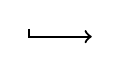
\begin{tikzpicture}
	\draw [->, thick] (0.2,0.2) -- (0.2,0.1) -- (1,0.1);
	\end{tikzpicture} & \hyperlink{R-3F7.1}{R-3F7.1} & \hyperlink{server::app::App}{server::app::App}
	
	\hyperlink{server::data::Questionnaire}{server::data::Questionnaire}
	
	\hyperlink{server::data::Tag}{server::data::Tag}
	
	\hyperlink{server::service::QuestionService}{server::service::QuestionService}
	
	\hyperlink{server::service::QuestionnaireService}{server::service::QuestionnaireService}
	
	\hyperlink{server::service::TagService}{server::service::TagService}\tabularnewline
	\hline
	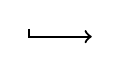
\begin{tikzpicture}
	\draw [->, thick] (0.2,0.2) -- (0.2,0.1) -- (1,0.1);
	\end{tikzpicture} & \hyperlink{R-3F7.2}{R-3F7.2} & \hyperlink{client::model::data::CurrentQuestion}{client::model::data::CurrentQuestion}
	
	\hyperlink{server::app::App}{server::app::App}
	
	\hyperlink{server::data::Question}{server::data::Question}
	
	\hyperlink{server::validator::QuestionCheck}{server::validator::QuestionCheck}\tabularnewline
	\hline
	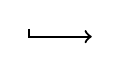
\begin{tikzpicture}
	\draw [->, thick] (0.2,0.2) -- (0.2,0.1) -- (1,0.1);
	\end{tikzpicture} & \hyperlink{R-3F7.3}{R-3F7.3} & \hyperlink{server::app::App}{server::app::App}
	
	\hyperlink{server::data::Questionnaire}{server::data::Questionnaire}
	
	\hyperlink{server::service::QuestionnaireService}{server::service::QuestionnaireService}
	
	\hyperlink{server::validator::QuestionnaireCheck}{server::validator::QuestionnaireCheck}\tabularnewline
	\hline
	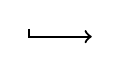
\begin{tikzpicture}
	\draw [->, thick] (0.2,0.2) -- (0.2,0.1) -- (1,0.1);
	\end{tikzpicture} & \hyperlink{R-3F7.4}{R-3F7.4} & \hyperlink{client::controller::student::ExecuteQuestionnaire}{client::controller::student::ExecuteQuestionnaire}
	
	\hyperlink{client::controller::student::ExecuteQuestion}{client::controller::student::ExecuteQuestion}
	
	\hyperlink{client::model::data::User}{client::model::data::User}
	
	\hyperlink{client::model::service::QuestionService}{client::model::service::QuestionService}
	
	\hyperlink{client::model::service::QuestionnaireService}{client::model::service::QuestionnaireService}
	
	\hyperlink{client::view::student::ExecuteQuestionnaire}{client::view::student::ExecuteQuestionnaire}
	
	\hyperlink{client::view::student::ExecuteQuestion}{client::view::student::ExecuteQuestion}
	
	\hyperlink{server::app::App}{server::app::App}\tabularnewline
	\hline
	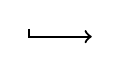
\begin{tikzpicture}
	\draw [->, thick] (0.2,0.2) -- (0.2,0.1) -- (1,0.1);
	\end{tikzpicture} & \hyperlink{R-3F7.5}{R-3F7.5} & \hyperlink{client::controller::teacher::ManipulateQuestion}{client::controller::teacher::ManipulateQuestion}
	
	\hyperlink{client::view::teacher::ManipulateQuestion}{client::view::teacher::ManipulateQuestion}
	
	\hyperlink{server::app::App}{server::app::App}
	
	\hyperlink{server::data::Question}{server::data::Question}
	
	\hyperlink{server::service::QuestionService}{server::service::QuestionService}
	
	\hyperlink{server::validator::QuestionCheck}{server::validator::QuestionCheck}\tabularnewline
	\hline
	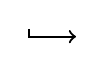
\begin{tikzpicture}
	\draw [->, thick] (0.4,0.2) -- (0.4,0.1) -- (1,0.1);
	\end{tikzpicture} & \hyperlink{R-3F7.5.1}{R-3F7.5.1} & \hyperlink{client::model::data::CurrentQuestion}{client::model::data::CurrentQuestion}
	
	\hyperlink{client::model::data::Question}{client::model::data::Question}
	
	\hyperlink{client::util::Check}{client::util::Check}
	
	\hyperlink{server::app::App}{server::app::App}
	
	\hyperlink{server::data::Question}{server::data::Question}
	
	\hyperlink{server::validator::QuestionCheck}{server::validator::QuestionCheck}\tabularnewline
	\hline
	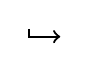
\begin{tikzpicture}
	\draw [->, thick] (0.6,0.2) -- (0.6,0.1) -- (1,0.1);
	\end{tikzpicture} & \hyperlink{R-3F7.5.1.2}{R-3F7.5.1.2} & \hyperlink{server::app::App}{server::app::App}
	
	\hyperlink{server::data::Question}{server::data::Question}
	
	\hyperlink{server::service::QuestionService}{server::service::QuestionService}
	
	\hyperlink{server::validator::QuestionCheck}{server::validator::QuestionCheck}\tabularnewline
	\hline
	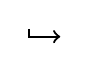
\begin{tikzpicture}
	\draw [->, thick] (0.6,0.2) -- (0.6,0.1) -- (1,0.1);
	\end{tikzpicture} & \hyperlink{R-3F7.5.1.6}{R-3F7.5.1.6} & \hyperlink{server::app::App}{server::app::App}
	
	\hyperlink{server::data::Question}{server::data::Question}
	
	\hyperlink{server::service::QuestionService}{server::service::QuestionService}
	
	\hyperlink{server::validator::QuestionCheck}{server::validator::QuestionCheck}\tabularnewline
	\hline
	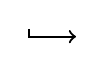
\begin{tikzpicture}
	\draw [->, thick] (0.4,0.2) -- (0.4,0.1) -- (1,0.1);
	\end{tikzpicture} & \hyperlink{R-3F7.5.3}{R-3F7.5.3} & \hyperlink{client::controller::student::ExecuteQuestionnaire}{client::controller::student::ExecuteQuestionnaire}
	
	\hyperlink{client::controller::student::ExecuteQuestion}{client::controller::student::ExecuteQuestion}
	
	\hyperlink{client::model::data::CurrentQuestion}{client::model::data::CurrentQuestion}
	
	\hyperlink{client::model::service::QuestionService}{client::model::service::QuestionService}
	
	\hyperlink{client::view::student::ExecuteQuestionnaire}{client::view::student::ExecuteQuestionnaire}
	
	\hyperlink{client::view::student::ExecuteQuestion}{client::view::student::ExecuteQuestion}
	
	\hyperlink{server::app::App}{server::app::App}
	
	\hyperlink{server::data::Question}{server::data::Question}
	
	\hyperlink{server::service::QuestionService}{server::service::QuestionService}
	
	\hyperlink{server::validator::QuestionCheck}{server::validator::QuestionCheck}\tabularnewline
	\hline
	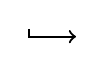
\begin{tikzpicture}
	\draw [->, thick] (0.4,0.2) -- (0.4,0.1) -- (1,0.1);
	\end{tikzpicture} & \hyperlink{R-3F7.5.5}{R-3F7.5.5} & \hyperlink{server::app::App}{server::app::App}
	
	\hyperlink{server::data::Question}{server::data::Question}
	
	\hyperlink{server::service::QuestionService}{server::service::QuestionService}
	
	\hyperlink{server::validator::QuestionCheck}{server::validator::QuestionCheck}\tabularnewline
	\hline
	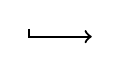
\begin{tikzpicture}
	\draw [->, thick] (0.2,0.2) -- (0.2,0.1) -- (1,0.1);
	\end{tikzpicture} & \hyperlink{R-3F7.7}{R-3F7.7} & \hyperlink{client::controller::teacher::ManipulateQuestionnaire}{client::controller::teacher::ManipulateQuestionnaire}
	
	\hyperlink{client::model::data::CurrentQuestionnaire}{client::model::data::CurrentQuestionnaire}
	
	\hyperlink{client::model::data::CurrentQuestion}{client::model::data::CurrentQuestion}
	
	\hyperlink{client::model::data::User}{client::model::data::User}
	
	\hyperlink{client::model::service::QuestionnaireService}{client::model::service::QuestionnaireService}
	
	\hyperlink{client::view::teacher::ManipulateQuestionnaire}{client::view::teacher::ManipulateQuestionnaire}
	
	\hyperlink{server::app::App}{server::app::App}
	
	\hyperlink{server::data::Questionnaire}{server::data::Questionnaire}
	
	\hyperlink{server::data::Question}{server::data::Question}
	
	\hyperlink{server::service::QuestionService}{server::service::QuestionService}
	
	\hyperlink{server::service::QuestionnaireService}{server::service::QuestionnaireService}
	
	\hyperlink{server::validator::QuestionCheck}{server::validator::QuestionCheck}
	
	\hyperlink{server::validator::QuestionnaireCheck}{server::validator::QuestionnaireCheck}\tabularnewline
	\hline
	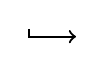
\begin{tikzpicture}
	\draw [->, thick] (0.4,0.2) -- (0.4,0.1) -- (1,0.1);
	\end{tikzpicture} & \hyperlink{R-3F7.7.1}{R-3F7.7.1} & \hyperlink{client::controller::teacher::ManipulateQuestionnaire}{client::controller::teacher::ManipulateQuestionnaire}
	
	\hyperlink{client::model::data::Questionnaire}{client::model::data::Questionnaire}
	
	\hyperlink{client::model::service::QuestionnaireService}{client::model::service::QuestionnaireService}
	
	\hyperlink{client::view::teacher::ManipulateQuestionnaire}{client::view::teacher::ManipulateQuestionnaire}
	
	\hyperlink{server::app::App}{server::app::App}
	
	\hyperlink{server::data::Questionnaire}{server::data::Questionnaire}
	
	\hyperlink{server::middleware::Authorization}{server::middleware::Authorization}
	
	\hyperlink{server::middleware::ErrorHandler}{server::middleware::ErrorHandler}
	
	\hyperlink{server::service::QuestionnaireService}{server::service::QuestionnaireService}
	
	\hyperlink{server::validator::QuestionnaireCheck}{server::validator::QuestionnaireCheck}\tabularnewline
	\hline
	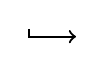
\begin{tikzpicture}
	\draw [->, thick] (0.4,0.2) -- (0.4,0.1) -- (1,0.1);
	\end{tikzpicture} & \hyperlink{R-2F7.10.3}{R-2F7.10.3} & \hyperlink{client::controller::user::Welcome}{client::controller::user::Welcome}
	
	\hyperlink{client::model::service::AnswerService}{client::model::service::AnswerService}
	
	\hyperlink{client::view::user::Welcome}{client::view::user::Welcome}
	
	\hyperlink{server::data::Answer}{server::data::Answer}
	
	\hyperlink{server::service::AnswerService}{server::service::AnswerService}
	
	\hyperlink{server::validator::AnswerCheck}{server::validator::AnswerCheck}\tabularnewline
	\hline
	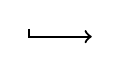
\begin{tikzpicture}
	\draw [->, thick] (0.2,0.2) -- (0.2,0.1) -- (1,0.1);
	\end{tikzpicture} & \hyperlink{R-3F7.11}{R-3F7.11} & \hyperlink{client::controller::teacher::ManageQuestions}{client::controller::teacher::ManageQuestions}
	
	\hyperlink{client::view::teacher::ManageQuestions}{client::view::teacher::ManageQuestions}
	
	\hyperlink{server::app::App}{server::app::App}
	
	\hyperlink{server::data::Question}{server::data::Question}
	
	\hyperlink{server::middleware::Authorization}{server::middleware::Authorization}
	
	\hyperlink{server::service::QuestionService}{server::service::QuestionService}
	
	\hyperlink{server::validator::QuestionCheck}{server::validator::QuestionCheck}\tabularnewline
	\hline
	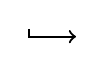
\begin{tikzpicture}
	\draw [->, thick] (0.4,0.2) -- (0.4,0.1) -- (1,0.1);
	\end{tikzpicture} & \hyperlink{R-3F7.11.1}{R-3F7.11.1} & \hyperlink{client::controller::teacher::ManageQuestions}{client::controller::teacher::ManageQuestions}
	
	\hyperlink{client::model::service::QuestionService}{client::model::service::QuestionService}
	
	\hyperlink{client::view::teacher::ManageQuestions}{client::view::teacher::ManageQuestions}
	
	\hyperlink{server::app::App}{server::app::App}
	
	\hyperlink{server::data::Question}{server::data::Question}
	
	\hyperlink{server::service::QuestionService}{server::service::QuestionService}
	
	\hyperlink{server::validator::QuestionCheck}{server::validator::QuestionCheck}\tabularnewline
	\hline
	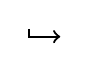
\begin{tikzpicture}
	\draw [->, thick] (0.6,0.2) -- (0.6,0.1) -- (1,0.1);
	\end{tikzpicture} & \hyperlink{R-3F7.11.1.1}{R-3F7.11.1.1} & \hyperlink{client::controller::teacher::ManipulateQuestion}{client::controller::teacher::ManipulateQuestion}
	
	\hyperlink{client::view::teacher::ManipulateQuestion}{client::view::teacher::ManipulateQuestion}
	
	\hyperlink{server::app::App}{server::app::App}
	
	\hyperlink{server::data::Question}{server::data::Question}
	
	\hyperlink{server::data::Tag}{server::data::Tag}
	
	\hyperlink{server::middleware::Authorization}{server::middleware::Authorization}
	
	\hyperlink{server::service::QuestionService}{server::service::QuestionService}
	
	\hyperlink{server::service::TagService}{server::service::TagService}\tabularnewline
	\hline
	\begin{tikzpicture}
	\draw [->, thick] (0.8,0.2) -- (0.8,0.1) -- (1,0.1);
	\end{tikzpicture} & \hyperlink{R-3F7.11.1.1.1}{R-3F7.11.1.1.1} & \hyperlink{client::controller::teacher::ManipulateQuestion}{client::controller::teacher::ManipulateQuestion}
	
	\hyperlink{client::view::teacher::ManipulateQuestion}{client::view::teacher::ManipulateQuestion}
	
	\hyperlink{server::app::App}{server::app::App}
	
	\hyperlink{server::data::Question}{server::data::Question}
	
	\hyperlink{server::data::Tag}{server::data::Tag}
	
	\hyperlink{server::middleware::Authorization}{server::middleware::Authorization}
	
	\hyperlink{server::middleware::ErrorHandler}{server::middleware::ErrorHandler}
	
	\hyperlink{server::service::QuestionService}{server::service::QuestionService}
	
	\hyperlink{server::service::TagService}{server::service::TagService}
	
	\hyperlink{server::validator::QuestionCheck}{server::validator::QuestionCheck}\tabularnewline
	\hline
	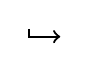
\begin{tikzpicture}
	\draw [->, thick] (0.6,0.2) -- (0.6,0.1) -- (1,0.1);
	\end{tikzpicture} & \hyperlink{R-3F7.11.1.2}{R-3F7.11.1.2} & \hyperlink{client::controller::teacher::ManipulateQuestion}{client::controller::teacher::ManipulateQuestion}
	
	\hyperlink{client::model::service::QuestionService}{client::model::service::QuestionService}
	
	\hyperlink{client::view::teacher::ManipulateQuestion}{client::view::teacher::ManipulateQuestion}
	
	\hyperlink{server::app::App}{server::app::App}
	
	\hyperlink{server::data::Question}{server::data::Question}
	
	\hyperlink{server::middleware::Authorization}{server::middleware::Authorization}
	
	\hyperlink{server::service::QuestionService}{server::service::QuestionService}
	
	\hyperlink{server::validator::QuestionCheck}{server::validator::QuestionCheck}\tabularnewline
	\hline
	\begin{tikzpicture}
	\draw [->, thick] (0.8,0.2) -- (0.8,0.1) -- (1,0.1);
	\end{tikzpicture} & \hyperlink{R-3F7.11.1.2.1}{R-3F7.11.1.2.1} & \hyperlink{client::controller::teacher::ManipulateQuestion}{client::controller::teacher::ManipulateQuestion}
	
	\hyperlink{client::model::service::QuestionService}{client::model::service::QuestionService}
	
	\hyperlink{client::view::teacher::ManipulateQuestion}{client::view::teacher::ManipulateQuestion}
	
	\hyperlink{server::app::App}{server::app::App}
	
	\hyperlink{server::data::Question}{server::data::Question}
	
	\hyperlink{server::middleware::Authorization}{server::middleware::Authorization}
	
	\hyperlink{server::middleware::ErrorHandler}{server::middleware::ErrorHandler}
	
	\hyperlink{server::service::QuestionService}{server::service::QuestionService}
	
	\hyperlink{server::validator::QuestionCheck}{server::validator::QuestionCheck}\tabularnewline
	\hline
	\begin{tikzpicture}
	\draw [->, thick] (0.8,0.2) -- (0.8,0.1) -- (1,0.1);
	\end{tikzpicture} & \hyperlink{R-3F7.11.1.2.2}{R-3F7.11.1.2.2} & \hyperlink{client::controller::teacher::ManipulateQuestion}{client::controller::teacher::ManipulateQuestion}
	
	\hyperlink{client::view::teacher::ManipulateQuestion}{client::view::teacher::ManipulateQuestion}
	
	\hyperlink{server::app::App}{server::app::App}
	
	\hyperlink{server::data::Question}{server::data::Question}
	
	\hyperlink{server::service::QuestionService}{server::service::QuestionService}
	
	\hyperlink{server::validator::QuestionCheck}{server::validator::QuestionCheck}\tabularnewline
	\hline
	\begin{tikzpicture}
	\draw [->, thick] (0.8,0.2) -- (0.8,0.1) -- (1,0.1);
	\end{tikzpicture} & \hyperlink{R-3F7.11.1.2.3}{R-3F7.11.1.2.3} & \hyperlink{client::controller::teacher::ManipulateQuestion}{client::controller::teacher::ManipulateQuestion}
	
	\hyperlink{client::model::service::QuestionService}{client::model::service::QuestionService}
	
	\hyperlink{client::view::teacher::ManipulateQuestion}{client::view::teacher::ManipulateQuestion}
	
	\hyperlink{server::app::App}{server::app::App}
	
	\hyperlink{server::data::Question}{server::data::Question}
	
	\hyperlink{server::middleware::Authorization}{server::middleware::Authorization}
	
	\hyperlink{server::service::QuestionService}{server::service::QuestionService}
	
	\hyperlink{server::validator::QuestionCheck}{server::validator::QuestionCheck}\tabularnewline
	\hline
	\begin{tikzpicture}
	\draw [->, thick] (0.8,0.2) -- (0.8,0.1) -- (1,0.1);
	\end{tikzpicture} & \hyperlink{R-1F7.11.1.2.4}{R-1F7.11.1.2.4} & \hyperlink{server::data::Question}{server::data::Question}
	
	\hyperlink{server::middleware::Authorization}{server::middleware::Authorization}
	
	\hyperlink{server::service::QuestionService}{server::service::QuestionService}
	
	\hyperlink{server::validator::QuestionCheck}{server::validator::QuestionCheck}\tabularnewline
	\hline
	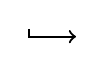
\begin{tikzpicture}
	\draw [->, thick] (0.4,0.2) -- (0.4,0.1) -- (1,0.1);
	\end{tikzpicture} & \hyperlink{R-3F7.11.2}{R-3F7.11.2} & \hyperlink{client::controller::teacher::ManipulateQuestion}{client::controller::teacher::ManipulateQuestion}
	
	\hyperlink{client::view::teacher::ManipulateQuestion}{client::view::teacher::ManipulateQuestion}
	
	\hyperlink{server::app::App}{server::app::App}
	
	\hyperlink{server::data::Question}{server::data::Question}
	
	\hyperlink{server::middleware::Authorization}{server::middleware::Authorization}
	
	\hyperlink{server::service::QuestionService}{server::service::QuestionService}
	
	\hyperlink{server::validator::QuestionCheck}{server::validator::QuestionCheck}\tabularnewline
	\hline
	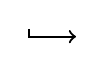
\begin{tikzpicture}
	\draw [->, thick] (0.4,0.2) -- (0.4,0.1) -- (1,0.1);
	\end{tikzpicture} & \hyperlink{R-3F7.11.3}{R-3F7.11.3} & \hyperlink{client::controller::teacher::ManageQuestions}{client::controller::teacher::ManageQuestions}
	
	\hyperlink{client::model::data::CurrentQuestion}{client::model::data::CurrentQuestion}
	
	\hyperlink{client::model::service::QuestionService}{client::model::service::QuestionService}
	
	\hyperlink{client::view::teacher::ManageQuestions}{client::view::teacher::ManageQuestions}
	
	\hyperlink{server::app::App}{server::app::App}
	
	\hyperlink{server::data::Question}{server::data::Question}
	
	\hyperlink{server::middleware::Authorization}{server::middleware::Authorization}
	
	\hyperlink{server::service::QuestionService}{server::service::QuestionService}\tabularnewline
	\hline
	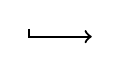
\begin{tikzpicture}
	\draw [->, thick] (0.2,0.2) -- (0.2,0.1) -- (1,0.1);
	\end{tikzpicture} & \hyperlink{R-3F7.12}{R-3F7.12} & \hyperlink{client::controller::teacher::ManipulateQuestionnaire}{client::controller::teacher::ManipulateQuestionnaire}
	
	\hyperlink{client::controller::teacher::SelectQuestion}{client::controller::teacher::SelectQuestion}
	
	\hyperlink{client::view::teacher::ManipulateQuestionnaire}{client::view::teacher::ManipulateQuestionnaire}
	
	\hyperlink{client::view::teacher::SelectQuestion}{client::view::teacher::SelectQuestion}
	
	\hyperlink{server::app::App}{server::app::App}
	
	\hyperlink{server::data::Questionnaire}{server::data::Questionnaire}
	
	\hyperlink{server::middleware::Authorization}{server::middleware::Authorization}
	
	\hyperlink{server::service::QuestionnaireService}{server::service::QuestionnaireService}
	
	\hyperlink{server::validator::QuestionnaireCheck}{server::validator::QuestionnaireCheck}\tabularnewline
	\hline
	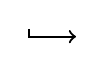
\begin{tikzpicture}
	\draw [->, thick] (0.4,0.2) -- (0.4,0.1) -- (1,0.1);
	\end{tikzpicture} & \hyperlink{R-3F7.12.1}{R-3F7.12.1} & \hyperlink{client::controller::teacher::ManageQuestionnaires}{client::controller::teacher::ManageQuestionnaires}
	
	\hyperlink{client::view::teacher::ManageQuestionnaires}{client::view::teacher::ManageQuestionnaires}
	
	\hyperlink{server::app::App}{server::app::App}
	
	\hyperlink{server::data::Questionnaire}{server::data::Questionnaire}
	
	\hyperlink{server::service::QuestionnaireService}{server::service::QuestionnaireService}\tabularnewline
	\hline
	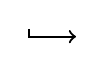
\begin{tikzpicture}
	\draw [->, thick] (0.4,0.2) -- (0.4,0.1) -- (1,0.1);
	\end{tikzpicture} & \hyperlink{R-3F7.12.2}{R-3F7.12.2} & \hyperlink{client::controller::teacher::ManipulateQuestionnaire}{client::controller::teacher::ManipulateQuestionnaire}
	
	\hyperlink{client::model::data::CurrentQuestionnaire}{client::model::data::CurrentQuestionnaire}
	
	\hyperlink{client::model::service::QuestionnaireService}{client::model::service::QuestionnaireService}
	
	\hyperlink{client::view::teacher::ManipulateQuestionnaire}{client::view::teacher::ManipulateQuestionnaire}
	
	\hyperlink{server::app::App}{server::app::App}
	
	\hyperlink{server::data::Questionnaire}{server::data::Questionnaire}
	
	\hyperlink{server::data::Question}{server::data::Question}
	
	\hyperlink{server::middleware::Authorization}{server::middleware::Authorization}
	
	\hyperlink{server::service::QuestionService}{server::service::QuestionService}
	
	\hyperlink{server::service::QuestionnaireService}{server::service::QuestionnaireService}
	
	\hyperlink{server::validator::QuestionnaireCheck}{server::validator::QuestionnaireCheck}\tabularnewline
	\hline
	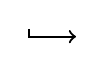
\begin{tikzpicture}
	\draw [->, thick] (0.4,0.2) -- (0.4,0.1) -- (1,0.1);
	\end{tikzpicture} & \hyperlink{R-3F7.12.3}{R-3F7.12.3} & \hyperlink{client::controller::teacher::ManageQuestionnaires}{client::controller::teacher::ManageQuestionnaires}
	
	\hyperlink{client::model::data::CurrentQuestionnaire}{client::model::data::CurrentQuestionnaire}
	
	\hyperlink{client::model::data::User}{client::model::data::User}
	
	\hyperlink{client::model::service::QuestionnaireService}{client::model::service::QuestionnaireService}
	
	\hyperlink{client::view::teacher::ManageQuestionnaires}{client::view::teacher::ManageQuestionnaires}
	
	\hyperlink{server::app::App}{server::app::App}
	
	\hyperlink{server::data::Questionnaire}{server::data::Questionnaire}
	
	\hyperlink{server::middleware::ErrorHandler}{server::middleware::ErrorHandler}
	
	\hyperlink{server::service::QuestionnaireService}{server::service::QuestionnaireService}\tabularnewline
	\hline
	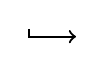
\begin{tikzpicture}
	\draw [->, thick] (0.4,0.2) -- (0.4,0.1) -- (1,0.1);
	\end{tikzpicture} & \hyperlink{R-3F7.12.4}{R-3F7.12.4} & \hyperlink{client::controller::teacher::ManipulateQuestionnaire}{client::controller::teacher::ManipulateQuestionnaire}
	
	\hyperlink{client::view::teacher::ManipulateQuestionnaire}{client::view::teacher::ManipulateQuestionnaire}
	
	\hyperlink{server::app::App}{server::app::App}
	
	\hyperlink{server::data::Questionnaire}{server::data::Questionnaire}
	
	\hyperlink{server::data::Tag}{server::data::Tag}
	
	\hyperlink{server::middleware::Authorization}{server::middleware::Authorization}
	
	\hyperlink{server::service::QuestionnaireService}{server::service::QuestionnaireService}
	
	\hyperlink{server::service::TagService}{server::service::TagService}
	
	\hyperlink{server::validator::QuestionnaireCheck}{server::validator::QuestionnaireCheck}\tabularnewline
	\hline
	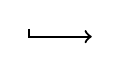
\begin{tikzpicture}
	\draw [->, thick] (0.2,0.2) -- (0.2,0.1) -- (1,0.1);
	\end{tikzpicture} & \hyperlink{R-3F7.13}{R-3F7.13} & \hyperlink{client::controller::teacher::ManageQuestionnaires}{client::controller::teacher::ManageQuestionnaires}
	
	\hyperlink{client::view::teacher::ManageQuestionnaires}{client::view::teacher::ManageQuestionnaires}
	
	\hyperlink{server::app::App}{server::app::App}
	
	\hyperlink{server::middleware::Authorization}{server::middleware::Authorization}
	
	\hyperlink{server::service::QuestionnaireService}{server::service::QuestionnaireService}\tabularnewline
	\hline
	& \hyperlink{R-3F8}{R-3F8} & \hyperlink{client::model::data::Role}{client::model::data::Role}
	
	\hyperlink{client::model::data::User}{client::model::data::User}
	
	\hyperlink{client::model::service::RoleService}{client::model::service::RoleService}
	
	\hyperlink{server::app::App}{server::app::App}
	
	\hyperlink{server::data::Role}{server::data::Role}
	
	\hyperlink{server::data::User}{server::data::User}
	
	\hyperlink{server::middleware::Authorization}{server::middleware::Authorization}
	
	\hyperlink{server::service::UserService}{server::service::UserService}
	
	\hyperlink{server::validator::UserCheck}{server::validator::UserCheck}\tabularnewline
	\hline
	& \hyperlink{R-3F9}{R-3F9} & \hyperlink{client::controller::public::SignUp}{client::controller::public::SignUp}
	
	\hyperlink{client::view::public::SignUp}{client::view::public::SignUp}
	
	\hyperlink{server::app::App}{server::app::App}
	
	\hyperlink{server::data::User}{server::data::User}
	
	\hyperlink{server::service::UserService}{server::service::UserService}
	
	\hyperlink{server::validator::UserCheck}{server::validator::UserCheck}\tabularnewline
	\hline
	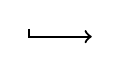
\begin{tikzpicture}
	\draw [->, thick] (0.2,0.2) -- (0.2,0.1) -- (1,0.1);
	\end{tikzpicture} & \hyperlink{R-3F9.1}{R-3F9.1} & \hyperlink{server::app::App}{server::app::App}
	
	\hyperlink{server::data::User}{server::data::User}
	
	\hyperlink{server::service::UserService}{server::service::UserService}
	
	\hyperlink{server::validator::UserCheck}{server::validator::UserCheck}\tabularnewline
	\hline
	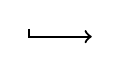
\begin{tikzpicture}
	\draw [->, thick] (0.2,0.2) -- (0.2,0.1) -- (1,0.1);
	\end{tikzpicture} & \hyperlink{R-3F9.2}{R-3F9.2} & \hyperlink{client::controller::public::SignUp}{client::controller::public::SignUp}
	
	\hyperlink{client::model::data::User}{client::model::data::User}
	
	\hyperlink{client::view::public::SignUp}{client::view::public::SignUp}
	
	\hyperlink{server::app::App}{server::app::App}
	
	\hyperlink{server::data::User}{server::data::User}
	
	\hyperlink{server::service::UserService}{server::service::UserService}
	
	\hyperlink{server::validator::UserCheck}{server::validator::UserCheck}\tabularnewline
	\hline
	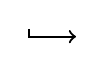
\begin{tikzpicture}
	\draw [->, thick] (0.4,0.2) -- (0.4,0.1) -- (1,0.1);
	\end{tikzpicture} & \hyperlink{R-3F9.2.1}{R-3F9.2.1} & \hyperlink{client::controller::public::SignUp}{client::controller::public::SignUp}
	
	\hyperlink{client::view::public::SignUp}{client::view::public::SignUp}
	
	\hyperlink{server::app::App}{server::app::App}
	
	\hyperlink{server::data::User}{server::data::User}
	
	\hyperlink{server::middleware::ErrorHandler}{server::middleware::ErrorHandler}
	
	\hyperlink{server::service::UserService}{server::service::UserService}
	
	\hyperlink{server::validator::UserCheck}{server::validator::UserCheck}\tabularnewline
	\hline
	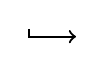
\begin{tikzpicture}
	\draw [->, thick] (0.4,0.2) -- (0.4,0.1) -- (1,0.1);
	\end{tikzpicture} & \hyperlink{R-3F9.2.2}{R-3F9.2.2} & \hyperlink{client::controller::public::SignUp}{client::controller::public::SignUp}
	
	\hyperlink{client::view::public::SignUp}{client::view::public::SignUp}
	
	\hyperlink{server::app::App}{server::app::App}
	
	\hyperlink{server::data::User}{server::data::User}
	
	\hyperlink{server::middleware::ErrorHandler}{server::middleware::ErrorHandler}
	
	\hyperlink{server::service::UserService}{server::service::UserService}
	
	\hyperlink{server::validator::UserCheck}{server::validator::UserCheck}\tabularnewline
	\hline
	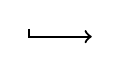
\begin{tikzpicture}
	\draw [->, thick] (0.2,0.2) -- (0.2,0.1) -- (1,0.1);
	\end{tikzpicture} & \hyperlink{R-3F9.3}{R-3F9.3} & \hyperlink{client::controller::public::SignUp}{client::controller::public::SignUp}
	
	\hyperlink{client::model::data::User}{client::model::data::User}
	
	\hyperlink{client::model::service::UserService}{client::model::service::UserService}
	
	\hyperlink{client::util::Check}{client::util::Check}
	
	\hyperlink{client::view::public::SignUp}{client::view::public::SignUp}
	
	\hyperlink{server::app::App}{server::app::App}
	
	\hyperlink{server::middleware::ErrorHandler}{server::middleware::ErrorHandler}
	
	\hyperlink{server::service::UserService}{server::service::UserService}
	
	\hyperlink{server::validator::UserCheck}{server::validator::UserCheck}\tabularnewline
	\hline
	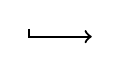
\begin{tikzpicture}
	\draw [->, thick] (0.2,0.2) -- (0.2,0.1) -- (1,0.1);
	\end{tikzpicture} & \hyperlink{R-3F9.4}{R-3F9.4} & \hyperlink{client::util::Check}{client::util::Check}
	
	\hyperlink{server::app::App}{server::app::App}
	
	\hyperlink{server::middleware::ErrorHandler}{server::middleware::ErrorHandler}
	
	\hyperlink{server::service::UserService}{server::service::UserService}
	
	\hyperlink{server::validator::UserCheck}{server::validator::UserCheck}\tabularnewline
	\hline
	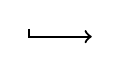
\begin{tikzpicture}
	\draw [->, thick] (0.2,0.2) -- (0.2,0.1) -- (1,0.1);
	\end{tikzpicture} & \hyperlink{R-3F9.5}{R-3F9.5} & \hyperlink{client::controller::public::SignUp}{client::controller::public::SignUp}
	
	\hyperlink{client::model::service::UserService}{client::model::service::UserService}
	
	\hyperlink{client::view::public::SignUp}{client::view::public::SignUp}
	
	\hyperlink{server::app::App}{server::app::App}
	
	\hyperlink{server::data::User}{server::data::User}
	
	\hyperlink{server::middleware::ErrorHandler}{server::middleware::ErrorHandler}
	
	\hyperlink{server::service::UserService}{server::service::UserService}
	
	\hyperlink{server::validator::UserCheck}{server::validator::UserCheck}\tabularnewline
	\hline
	& \hyperlink{R-3F11}{R-3F11} & \hyperlink{client::controller::admin::UsersList}{client::controller::admin::UsersList}
	
	\hyperlink{client::view::admin::UsersList}{client::view::admin::UsersList}
	
	\hyperlink{server::app::App}{server::app::App}
	
	\hyperlink{server::data::Role}{server::data::Role}
	
	\hyperlink{server::data::User}{server::data::User}
	
	\hyperlink{server::service::RoleService}{server::service::RoleService}
	
	\hyperlink{server::service::UserService}{server::service::UserService}
	
	\hyperlink{server::validator::UserCheck}{server::validator::UserCheck}\tabularnewline
	\hline
	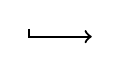
\begin{tikzpicture}
	\draw [->, thick] (0.2,0.2) -- (0.2,0.1) -- (1,0.1);
	\end{tikzpicture} & \hyperlink{R-3F11.1}{R-3F11.1} & \hyperlink{client::controller::admin::UsersList}{client::controller::admin::UsersList}
	
	\hyperlink{client::model::data::User}{client::model::data::User}
	
	\hyperlink{client::model::service::RoleService}{client::model::service::RoleService}
	
	\hyperlink{client::view::admin::UsersList}{client::view::admin::UsersList}
	
	\hyperlink{server::app::App}{server::app::App}
	
	\hyperlink{server::data::Role}{server::data::Role}
	
	\hyperlink{server::data::User}{server::data::User}
	
	\hyperlink{server::middleware::Authorization}{server::middleware::Authorization}
	
	\hyperlink{server::service::RoleService}{server::service::RoleService}
	
	\hyperlink{server::service::UserService}{server::service::UserService}
	
	\hyperlink{server::validator::UserCheck}{server::validator::UserCheck}\tabularnewline
	\hline
	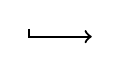
\begin{tikzpicture}
	\draw [->, thick] (0.2,0.2) -- (0.2,0.1) -- (1,0.1);
	\end{tikzpicture} & \hyperlink{R-3F11.2}{R-3F11.2} & \hyperlink{client::controller::admin::UsersList}{client::controller::admin::UsersList}
	
	\hyperlink{client::view::admin::UsersList}{client::view::admin::UsersList}
	
	\hyperlink{server::app::App}{server::app::App}
	
	\hyperlink{server::data::User}{server::data::User}
	
	\hyperlink{server::middleware::Authorization}{server::middleware::Authorization}
	
	\hyperlink{server::service::UserService}{server::service::UserService}\tabularnewline
	\hline
	& \hyperlink{R-3F13}{R-3F13} & \hyperlink{client::model::data::User}{client::model::data::User}
	
	\hyperlink{client::model::service::UserService}{client::model::service::UserService}
	
	\hyperlink{server::app::App}{server::app::App}
	
	\hyperlink{server::data::User}{server::data::User}
	
	\hyperlink{server::service::UserService}{server::service::UserService}
	
	\hyperlink{server::validator::UserCheck}{server::validator::UserCheck}\tabularnewline
	\hline
	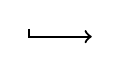
\begin{tikzpicture}
	\draw [->, thick] (0.2,0.2) -- (0.2,0.1) -- (1,0.1);
	\end{tikzpicture} & \hyperlink{R-3F13.1}{R-3F13.1} & \hyperlink{client::model::data::User}{client::model::data::User}
	
	\hyperlink{client::model::service::UserService}{client::model::service::UserService}
	
	\hyperlink{client::util::Check}{client::util::Check}
	
	\hyperlink{server::app::App}{server::app::App}
	
	\hyperlink{server::data::User}{server::data::User}
	
	\hyperlink{server::service::UserService}{server::service::UserService}
	
	\hyperlink{server::validator::UserCheck}{server::validator::UserCheck}\tabularnewline
	\hline
	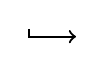
\begin{tikzpicture}
	\draw [->, thick] (0.4,0.2) -- (0.4,0.1) -- (1,0.1);
	\end{tikzpicture} & \hyperlink{R-3F13.1.1}{R-3F13.1.1} & \hyperlink{client::util::Check}{client::util::Check}
	
	\hyperlink{server::app::App}{server::app::App}
	
	\hyperlink{server::data::User}{server::data::User}
	
	\hyperlink{server::middleware::ErrorHandler}{server::middleware::ErrorHandler}
	
	\hyperlink{server::service::UserService}{server::service::UserService}
	
	\hyperlink{server::validator::UserCheck}{server::validator::UserCheck}\tabularnewline
	\hline
	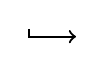
\begin{tikzpicture}
	\draw [->, thick] (0.4,0.2) -- (0.4,0.1) -- (1,0.1);
	\end{tikzpicture} & \hyperlink{R-3F13.1.2}{R-3F13.1.2} & \hyperlink{client::controller::public::SignUp}{client::controller::public::SignUp}
	
	\hyperlink{client::model::service::UserService}{client::model::service::UserService}
	
	\hyperlink{client::view::public::SignUp}{client::view::public::SignUp}
	
	\hyperlink{server::app::App}{server::app::App}
	
	\hyperlink{server::data::User}{server::data::User}
	
	\hyperlink{server::service::UserService}{server::service::UserService}
	
	\hyperlink{server::validator::UserCheck}{server::validator::UserCheck}\tabularnewline
	\hline
	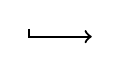
\begin{tikzpicture}
	\draw [->, thick] (0.2,0.2) -- (0.2,0.1) -- (1,0.1);
	\end{tikzpicture} & \hyperlink{R-3F13.2}{R-3F13.2} & \hyperlink{server::app::App}{server::app::App}
	
	\hyperlink{server::data::User}{server::data::User}
	
	\hyperlink{server::service::UserService}{server::service::UserService}
	
	\hyperlink{server::validator::UserCheck}{server::validator::UserCheck}\tabularnewline
	\hline
	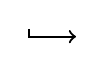
\begin{tikzpicture}
	\draw [->, thick] (0.4,0.2) -- (0.4,0.1) -- (1,0.1);
	\end{tikzpicture} & \hyperlink{R-3F13.2.1}{R-3F13.2.1} & \hyperlink{client::model::data::User}{client::model::data::User}
	
	\hyperlink{client::model::service::UserService}{client::model::service::UserService}
	
	\hyperlink{client::util::Check}{client::util::Check}
	
	\hyperlink{server::app::App}{server::app::App}
	
	\hyperlink{server::data::User}{server::data::User}
	
	\hyperlink{server::service::UserService}{server::service::UserService}
	
	\hyperlink{server::validator::UserCheck}{server::validator::UserCheck}\tabularnewline
	\hline
	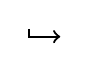
\begin{tikzpicture}
	\draw [->, thick] (0.6,0.2) -- (0.6,0.1) -- (1,0.1);
	\end{tikzpicture} & \hyperlink{R-3F13.2.1.1}{R-3F13.2.1.1} & \hyperlink{client::model::service::UserService}{client::model::service::UserService}
	
	\hyperlink{client::util::Check}{client::util::Check}
	
	\hyperlink{server::app::App}{server::app::App}
	
	\hyperlink{server::data::User}{server::data::User}
	
	\hyperlink{server::middleware::ErrorHandler}{server::middleware::ErrorHandler}
	
	\hyperlink{server::service::UserService}{server::service::UserService}
	
	\hyperlink{server::validator::UserCheck}{server::validator::UserCheck}\tabularnewline
	\hline
	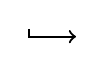
\begin{tikzpicture}
	\draw [->, thick] (0.4,0.2) -- (0.4,0.1) -- (1,0.1);
	\end{tikzpicture} & \hyperlink{R-3F13.2.2}{R-3F13.2.2} & \hyperlink{client::model::data::User}{client::model::data::User}
	
	\hyperlink{server::app::App}{server::app::App}
	
	\hyperlink{server::data::User}{server::data::User}
	
	\hyperlink{server::service::UserService}{server::service::UserService}
	
	\hyperlink{server::validator::UserCheck}{server::validator::UserCheck}\tabularnewline
	\hline
	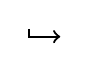
\begin{tikzpicture}
	\draw [->, thick] (0.6,0.2) -- (0.6,0.1) -- (1,0.1);
	\end{tikzpicture} & \hyperlink{R-3F13.2.2.1}{R-3F13.2.2.1} & \hyperlink{client::util::Check}{client::util::Check}
	
	\hyperlink{server::app::App}{server::app::App}
	
	\hyperlink{server::middleware::ErrorHandler}{server::middleware::ErrorHandler}
	
	\hyperlink{server::service::UserService}{server::service::UserService}
	
	\hyperlink{server::validator::UserCheck}{server::validator::UserCheck}\tabularnewline
	\hline
	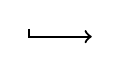
\begin{tikzpicture}
	\draw [->, thick] (0.2,0.2) -- (0.2,0.1) -- (1,0.1);
	\end{tikzpicture} & \hyperlink{R-3F13.3}{R-3F13.3} & \hyperlink{client::model::data::User}{client::model::data::User}
	
	\hyperlink{client::model::service::UserService}{client::model::service::UserService}
	
	\hyperlink{server::app::App}{server::app::App}
	
	\hyperlink{server::data::User}{server::data::User}
	
	\hyperlink{server::service::UserService}{server::service::UserService}
	
	\hyperlink{server::validator::UserCheck}{server::validator::UserCheck}\tabularnewline
	\hline
	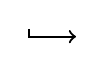
\begin{tikzpicture}
	\draw [->, thick] (0.4,0.2) -- (0.4,0.1) -- (1,0.1);
	\end{tikzpicture} & \hyperlink{R-3F13.3.1}{R-3F13.3.1} & \hyperlink{client::model::data::User}{client::model::data::User}
	
	\hyperlink{client::model::service::UserService}{client::model::service::UserService}
	
	\hyperlink{client::util::Check}{client::util::Check}
	
	\hyperlink{server::app::App}{server::app::App}
	
	\hyperlink{server::data::User}{server::data::User}
	
	\hyperlink{server::service::UserService}{server::service::UserService}
	
	\hyperlink{server::validator::UserCheck}{server::validator::UserCheck}\tabularnewline
	\hline
	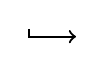
\begin{tikzpicture}
	\draw [->, thick] (0.4,0.2) -- (0.4,0.1) -- (1,0.1);
	\end{tikzpicture} & \hyperlink{R-3F13.3.2}{R-3F13.3.2} & \hyperlink{client::model::data::User}{client::model::data::User}
	
	\hyperlink{client::model::service::UserService}{client::model::service::UserService}
	
	\hyperlink{client::util::Check}{client::util::Check}
	
	\hyperlink{server::app::App}{server::app::App}
	
	\hyperlink{server::data::User}{server::data::User}
	
	\hyperlink{server::service::UserService}{server::service::UserService}
	
	\hyperlink{server::validator::UserCheck}{server::validator::UserCheck}\tabularnewline
	\hline
	\begin{tikzpicture}
	\draw [->, thick] (0.4,0.2) -- (0.4,0.1) -- (1,0.1);
	\end{tikzpicture} & \hyperlink{R-3F13.3.3}{R-3F13.3.3} & \hyperlink{server::app::App}{server::app::App}
	
	\hyperlink{server::data::User}{server::data::User}
	
	\hyperlink{server::middleware::ErrorHandler}{server::middleware::ErrorHandler}
	
	\hyperlink{server::service::UserService}{server::service::UserService}
	
	\hyperlink{server::validator::UserCheck}{server::validator::UserCheck}\tabularnewline
	\hline
	\begin{tikzpicture}
	\draw [->, thick] (0.4,0.2) -- (0.4,0.1) -- (1,0.1);
	\end{tikzpicture} & \hyperlink{R-3F13.3.4}{R-3F13.3.4} & \hyperlink{client::util::Check}{client::util::Check}
	
	\hyperlink{server::app::App}{server::app::App}
	
	\hyperlink{server::data::User}{server::data::User}
	
	\hyperlink{server::middleware::ErrorHandler}{server::middleware::ErrorHandler}
	
	\hyperlink{server::service::UserService}{server::service::UserService}
	
	\hyperlink{server::validator::UserCheck}{server::validator::UserCheck}\tabularnewline
	\hline
	& \hyperlink{R-3F14}{R-3F14} & \hyperlink{client::controller::teacher::ManageQuestionnaires}{client::controller::teacher::ManageQuestionnaires}
	
	\hyperlink{client::model::service::QuestionnaireService}{client::model::service::QuestionnaireService}
	
	\hyperlink{client::view::teacher::ManageQuestionnaires}{client::view::teacher::ManageQuestionnaires}
	
	\hyperlink{server::app::App}{server::app::App}
	
	\hyperlink{server::data::Questionnaire}{server::data::Questionnaire}
	
	\hyperlink{server::service::QuestionnaireService}{server::service::QuestionnaireService}\tabularnewline
	\hline
	\begin{tikzpicture}
	\draw [->, thick] (0.2,0.2) -- (0.2,0.1) -- (1,0.1);
	\end{tikzpicture} & \hyperlink{R-3F14.1}{R-3F14.1} & \hyperlink{client::controller::student::Questionnaires}{client::controller::student::Questionnaires}
	
	\hyperlink{client::view::student::Questionnaires}{client::view::student::Questionnaires}
	
	\hyperlink{server::app::App}{server::app::App}
	
	\hyperlink{server::data::Questionnaire}{server::data::Questionnaire}
	
	\hyperlink{server::service::QuestionnaireService}{server::service::QuestionnaireService}\tabularnewline
	\hline
	\begin{tikzpicture}
	\draw [->, thick] (0.2,0.2) -- (0.2,0.1) -- (1,0.1);
	\end{tikzpicture} & \hyperlink{R-3F14.3}{R-3F14.3} & \hyperlink{client::controller::student::Questionnaires}{client::controller::student::Questionnaires}
	
	\hyperlink{client::model::service::QuestionnaireService}{client::model::service::QuestionnaireService}
	
	\hyperlink{client::view::student::Questionnaires}{client::view::student::Questionnaires}
	
	\hyperlink{server::app::App}{server::app::App}
	
	\hyperlink{server::data::Questionnaire}{server::data::Questionnaire}
	
	\hyperlink{server::service::QuestionnaireService}{server::service::QuestionnaireService}\tabularnewline
	\hline
	\begin{tikzpicture}
	\draw [->, thick] (0.2,0.2) -- (0.2,0.1) -- (1,0.1);
	\end{tikzpicture} & \hyperlink{R-3F14.4}{R-3F14.4} & \hyperlink{client::controller::student::Questionnaires}{client::controller::student::Questionnaires}
	
	\hyperlink{client::view::student::Questionnaires}{client::view::student::Questionnaires}
	
	\hyperlink{server::app::App}{server::app::App}
	
	\hyperlink{server::data::Questionnaire}{server::data::Questionnaire}
	
	\hyperlink{server::data::Tag}{server::data::Tag}
	
	\hyperlink{server::service::QuestionnaireService}{server::service::QuestionnaireService}
	
	\hyperlink{server::service::TagService}{server::service::TagService}\tabularnewline
	\hline
	& \hyperlink{R-3F16}{R-3F16} & \hyperlink{client::controller::student::ExecuteQuestionnaire}{client::controller::student::ExecuteQuestionnaire}
	
	\hyperlink{client::controller::student::ExecuteQuestion}{client::controller::student::ExecuteQuestion}
	
	\hyperlink{client::model::data::CurrentQuestionnaire}{client::model::data::CurrentQuestionnaire}
	
	\hyperlink{client::model::data::CurrentQuestion}{client::model::data::CurrentQuestion}
	
	\hyperlink{client::model::data::User}{client::model::data::User}
	
	\hyperlink{client::view::student::ExecuteQuestionnaire}{client::view::student::ExecuteQuestionnaire}
	
	\hyperlink{client::view::student::ExecuteQuestion}{client::view::student::ExecuteQuestion}
	
	\hyperlink{server::app::App}{server::app::App}
	
	\hyperlink{server::data::Questionnaire}{server::data::Questionnaire}
	
	\hyperlink{server::service::QuestionnaireService}{server::service::QuestionnaireService}\tabularnewline
	\hline
	\begin{tikzpicture}
	\draw [->, thick] (0.2,0.2) -- (0.2,0.1) -- (1,0.1);
	\end{tikzpicture} & \hyperlink{R-3F16.1}{R-3F16.1} & \hyperlink{client::controller::student::ExecuteQuestion}{client::controller::student::ExecuteQuestion}
	
	\hyperlink{client::view::student::ExecuteQuestion}{client::view::student::ExecuteQuestion}
	
	\hyperlink{server::app::App}{server::app::App}
	
	\hyperlink{server::data::Question}{server::data::Question}
	
	\hyperlink{server::service::QuestionService}{server::service::QuestionService}\tabularnewline
	\hline
	\begin{tikzpicture}
	\draw [->, thick] (0.4,0.2) -- (0.4,0.1) -- (1,0.1);
	\end{tikzpicture} & \hyperlink{R-3F16.1.1}{R-3F16.1.1} & \hyperlink{client::controller::student::ExecuteQuestion}{client::controller::student::ExecuteQuestion}
	
	\hyperlink{client::view::student::ExecuteQuestion}{client::view::student::ExecuteQuestion}
	
	\hyperlink{server::app::App}{server::app::App}
	
	\hyperlink{server::data::Question}{server::data::Question}
	
	\hyperlink{server::service::QuestionService}{server::service::QuestionService}\tabularnewline
	\hline
	\begin{tikzpicture}
	\draw [->, thick] (0.4,0.2) -- (0.4,0.1) -- (1,0.1);
	\end{tikzpicture} & \hyperlink{R-3F16.1.2}{R-3F16.1.2} & \hyperlink{client::controller::student::ExecuteQuestion}{client::controller::student::ExecuteQuestion}
	
	\hyperlink{client::view::student::ExecuteQuestion}{client::view::student::ExecuteQuestion}
	
	\hyperlink{server::app::App}{server::app::App}
	
	\hyperlink{server::data::Question}{server::data::Question}
	
	\hyperlink{server::service::QuestionService}{server::service::QuestionService}\tabularnewline
	\hline
	\begin{tikzpicture}
	\draw [->, thick] (0.2,0.2) -- (0.2,0.1) -- (1,0.1);
	\end{tikzpicture} & \hyperlink{R-3F16.2}{R-3F16.2} & \hyperlink{client::controller::student::ExecuteQuestionnaire}{client::controller::student::ExecuteQuestionnaire}
	
	\hyperlink{client::view::student::ExecuteQuestionnaire}{client::view::student::ExecuteQuestionnaire}
	
	\hyperlink{server::app::App}{server::app::App}\tabularnewline
	\hline
	\begin{tikzpicture}
	\draw [->, thick] (0.4,0.2) -- (0.4,0.1) -- (1,0.1);
	\end{tikzpicture} & \hyperlink{R-3F16.2.1}{R-3F16.2.1} & \hyperlink{client::controller::student::ExecuteQuestionnaire}{client::controller::student::ExecuteQuestionnaire}
	
	\hyperlink{client::view::student::ExecuteQuestionnaire}{client::view::student::ExecuteQuestionnaire}
	
	\hyperlink{server::app::App}{server::app::App}\tabularnewline
	\hline
	\begin{tikzpicture}
	\draw [->, thick] (0.2,0.2) -- (0.2,0.1) -- (1,0.1);
	\end{tikzpicture} & \hyperlink{R-3F16.3}{R-3F16.3} & \hyperlink{client::controller::student::ExecuteQuestionnaire}{client::controller::student::ExecuteQuestionnaire}
	
	\hyperlink{client::model::data::CurrentQuestionnaire}{client::model::data::CurrentQuestionnaire}
	
	\hyperlink{client::model::data::CurrentQuestion}{client::model::data::CurrentQuestion}
	
	\hyperlink{client::view::student::ExecuteQuestionnaire}{client::view::student::ExecuteQuestionnaire}
	
	\hyperlink{server::app::App}{server::app::App}\tabularnewline
	\hline
	\begin{tikzpicture}
	\draw [->, thick] (0.2,0.2) -- (0.2,0.1) -- (1,0.1);
	\end{tikzpicture} & \hyperlink{R-3F16.4}{R-3F16.4} & \hyperlink{client::controller::student::ExecuteQuestionnaire}{client::controller::student::ExecuteQuestionnaire}
	
	\hyperlink{client::model::data::CurrentQuestionnaire}{client::model::data::CurrentQuestionnaire}
	
	\hyperlink{client::model::data::CurrentQuestion}{client::model::data::CurrentQuestion}
	
	\hyperlink{client::view::student::ExecuteQuestionnaire}{client::view::student::ExecuteQuestionnaire}
	
	\hyperlink{server::app::App}{server::app::App}\tabularnewline
	\hline
	& \hyperlink{R-3F17}{R-3F17} & \hyperlink{client::model::data::User}{client::model::data::User}
	
	\hyperlink{client::model::service::SessionService}{client::model::service::SessionService}
	
	\hyperlink{server::app::App}{server::app::App}
	
	\hyperlink{server::data::User}{server::data::User}
	
	\hyperlink{server::service::SessionService}{server::service::SessionService}\tabularnewline
	\hline
	& \hyperlink{R-3F18}{R-3F18} & \hyperlink{client::controller::admin::UsersList}{client::controller::admin::UsersList}
	
	\hyperlink{client::model::data::User}{client::model::data::User}
	
	\hyperlink{client::model::service::RoleService}{client::model::service::RoleService}
	
	\hyperlink{client::view::admin::UsersList}{client::view::admin::UsersList}
	
	\hyperlink{server::app::App}{server::app::App}
	
	\hyperlink{server::data::Role}{server::data::Role}
	
	\hyperlink{server::data::User}{server::data::User}
	
	\hyperlink{server::middleware::Authorization}{server::middleware::Authorization}
	
	\hyperlink{server::service::RoleService}{server::service::RoleService}
	
	\hyperlink{server::service::UserService}{server::service::UserService}\tabularnewline
	\hline
	\begin{tikzpicture}
	\draw [->, thick] (0.2,0.2) -- (0.2,0.1) -- (1,0.1);
	\end{tikzpicture} & \hyperlink{R-3F18.1}{R-3F18.1} & \hyperlink{client::controller::admin::UsersList}{client::controller::admin::UsersList}
	
	\hyperlink{client::model::service::RoleService}{client::model::service::RoleService}
	
	\hyperlink{client::view::admin::UsersList}{client::view::admin::UsersList}
	
	\hyperlink{server::app::App}{server::app::App}
	
	\hyperlink{server::data::User}{server::data::User}
	
	\hyperlink{server::service::UserService}{server::service::UserService}\tabularnewline
	\hline
	\begin{tikzpicture}
	\draw [->, thick] (0.2,0.2) -- (0.2,0.1) -- (1,0.1);
	\end{tikzpicture} & \hyperlink{R-3F18.2}{R-3F18.2} & \hyperlink{client::controller::admin::UsersList}{client::controller::admin::UsersList}
	
	\hyperlink{client::view::admin::UsersList}{client::view::admin::UsersList}
	
	\hyperlink{server::app::App}{server::app::App}
	
	\hyperlink{server::middleware::Authorization}{server::middleware::Authorization}\tabularnewline
	\hline
	\begin{tikzpicture}
	\draw [->, thick] (0.2,0.2) -- (0.2,0.1) -- (1,0.1);
	\end{tikzpicture} & \hyperlink{R-3F18.3}{R-3F18.3} & \hyperlink{client::controller::admin::UsersList}{client::controller::admin::UsersList}
	
	\hyperlink{client::view::admin::UsersList}{client::view::admin::UsersList}
	
	\hyperlink{server::app::App}{server::app::App}
	
	\hyperlink{server::middleware::Authorization}{server::middleware::Authorization}\tabularnewline
	\hline
	& \hyperlink{R-3F19}{R-3F19} & \hyperlink{client::controller::teacher::SelectQuestion}{client::controller::teacher::SelectQuestion}
	
	\hyperlink{client::view::teacher::SelectQuestion}{client::view::teacher::SelectQuestion}
	
	\hyperlink{server::app::App}{server::app::App}
	
	\hyperlink{server::data::Question}{server::data::Question}
	
	\hyperlink{server::middleware::Authorization}{server::middleware::Authorization}
	
	\hyperlink{server::service::QuestionService}{server::service::QuestionService}\tabularnewline
	\hline
	\begin{tikzpicture}
	\draw [->, thick] (0.2,0.2) -- (0.2,0.1) -- (1,0.1);
	\end{tikzpicture} & \hyperlink{R-3F19.1}{R-3F19.1} & \hyperlink{client::controller::teacher::SelectQuestion}{client::controller::teacher::SelectQuestion}
	
	\hyperlink{client::view::teacher::SelectQuestion}{client::view::teacher::SelectQuestion}
	
	\hyperlink{server::app::App}{server::app::App}
	
	\hyperlink{server::data::Question}{server::data::Question}
	
	\hyperlink{server::data::Tag}{server::data::Tag}
	
	\hyperlink{server::middleware::Authorization}{server::middleware::Authorization}
	
	\hyperlink{server::service::QuestionService}{server::service::QuestionService}
	
	\hyperlink{server::service::TagService}{server::service::TagService}\tabularnewline
	\hline
	\begin{tikzpicture}
	\draw [->, thick] (0.2,0.2) -- (0.2,0.1) -- (1,0.1);
	\end{tikzpicture} & \hyperlink{R-3F19.2}{R-3F19.2} & \hyperlink{client::controller::teacher::SelectQuestion}{client::controller::teacher::SelectQuestion}
	
	\hyperlink{client::view::teacher::SelectQuestion}{client::view::teacher::SelectQuestion}
	
	\hyperlink{server::app::App}{server::app::App}
	
	\hyperlink{server::data::Question}{server::data::Question}
	
	\hyperlink{server::middleware::Authorization}{server::middleware::Authorization}
	
	\hyperlink{server::service::QuestionService}{server::service::QuestionService}\tabularnewline
	\hline
	\begin{tikzpicture}
	\draw [->, thick] (0.2,0.2) -- (0.2,0.1) -- (1,0.1);
	\end{tikzpicture} & \hyperlink{R-3F19.4}{R-3F19.4} & \hyperlink{client::controller::teacher::SelectQuestion}{client::controller::teacher::SelectQuestion}
	
	\hyperlink{client::view::teacher::SelectQuestion}{client::view::teacher::SelectQuestion}
	
	\hyperlink{server::app::App}{server::app::App}
	
	\hyperlink{server::data::Question}{server::data::Question}
	
	\hyperlink{server::middleware::Authorization}{server::middleware::Authorization}
	
	\hyperlink{server::service::QuestionService}{server::service::QuestionService}\tabularnewline
	\hline
	& \hyperlink{R-3F22}{R-3F22} & \hyperlink{client::controller::teacher::ManageTags}{client::controller::teacher::ManageTags}
	
	\hyperlink{client::model::service::TagService}{client::model::service::TagService}
	
	\hyperlink{client::view::teacher::ManageTags}{client::view::teacher::ManageTags}
	
	\hyperlink{server::app::App}{server::app::App}
	
	\hyperlink{server::data::Tag}{server::data::Tag}
	
	\hyperlink{server::middleware::Authorization}{server::middleware::Authorization}
	
	\hyperlink{server::service::TagService}{server::service::TagService}
	
	\hyperlink{server::validator::TagCheck}{server::validator::TagCheck}\tabularnewline
	\hline
	\begin{tikzpicture}
	\draw [->, thick] (0.2,0.2) -- (0.2,0.1) -- (1,0.1);
	\end{tikzpicture} & \hyperlink{R-3F22.1}{R-3F22.1} & \hyperlink{client::model::data::Tag}{client::model::data::Tag}
	
	\hyperlink{server::app::App}{server::app::App}
	
	\hyperlink{server::data::Tag}{server::data::Tag}
	
	\hyperlink{server::middleware::Authorization}{server::middleware::Authorization}
	
	\hyperlink{server::service::TagService}{server::service::TagService}
	
	\hyperlink{server::validator::TagCheck}{server::validator::TagCheck}\tabularnewline
	\hline
	\begin{tikzpicture}
	\draw [->, thick] (0.4,0.2) -- (0.4,0.1) -- (1,0.1);
	\end{tikzpicture} & \hyperlink{R-3F22.1.1}{R-3F22.1.1} & \hyperlink{client::model::service::TagService}{client::model::service::TagService}
	
	\hyperlink{server::app::App}{server::app::App}
	
	\hyperlink{server::data::Tag}{server::data::Tag}
	
	\hyperlink{server::middleware::Authorization}{server::middleware::Authorization}
	
	\hyperlink{server::middleware::ErrorHandler}{server::middleware::ErrorHandler}
	
	\hyperlink{server::service::TagService}{server::service::TagService}
	
	\hyperlink{server::validator::TagCheck}{server::validator::TagCheck}\tabularnewline
	\hline
	\begin{tikzpicture}
	\draw [->, thick] (0.2,0.2) -- (0.2,0.1) -- (1,0.1);
	\end{tikzpicture} & \hyperlink{R-3F22.2}{R-3F22.2} & \hyperlink{client::controller::teacher::ManageTags}{client::controller::teacher::ManageTags}
	
	\hyperlink{client::model::data::Tag}{client::model::data::Tag}
	
	\hyperlink{client::view::teacher::ManageTags}{client::view::teacher::ManageTags}
	
	\hyperlink{server::app::App}{server::app::App}
	
	\hyperlink{server::data::Tag}{server::data::Tag}
	
	\hyperlink{server::middleware::Authorization}{server::middleware::Authorization}
	
	\hyperlink{server::service::TagService}{server::service::TagService}\tabularnewline
	\hline
	\begin{tikzpicture}
	\draw [->, thick] (0.4,0.2) -- (0.4,0.1) -- (1,0.1);
	\end{tikzpicture} & \hyperlink{R-3F22.2.1}{R-3F22.2.1} & \hyperlink{client::controller::teacher::ManageTags}{client::controller::teacher::ManageTags}
	
	\hyperlink{client::model::service::TagService}{client::model::service::TagService}
	
	\hyperlink{client::view::teacher::ManageTags}{client::view::teacher::ManageTags}
	
	\hyperlink{server::app::App}{server::app::App}
	
	\hyperlink{server::middleware::Authorization}{server::middleware::Authorization}
	
	\hyperlink{server::service::TagService}{server::service::TagService}\tabularnewline
	\hline
	\begin{tikzpicture}
	\draw [->, thick] (0.4,0.2) -- (0.4,0.1) -- (1,0.1);
	\end{tikzpicture} & \hyperlink{R-3F22.2.2}{R-3F22.2.2} & \hyperlink{client::model::service::TagService}{client::model::service::TagService}
	
	\hyperlink{server::app::App}{server::app::App}
	
	\hyperlink{server::middleware::Authorization}{server::middleware::Authorization}
	
	\hyperlink{server::service::TagService}{server::service::TagService}
	
	\hyperlink{server::validator::TagCheck}{server::validator::TagCheck}\tabularnewline
	\hline
	\begin{tikzpicture}
	\draw [->, thick] (0.2,0.2) -- (0.2,0.1) -- (1,0.1);
	\end{tikzpicture} & \hyperlink{R-3F22.3}{R-3F22.3} & \hyperlink{client::model::data::Tag}{client::model::data::Tag}
	
	\hyperlink{server::app::App}{server::app::App}
	
	\hyperlink{server::data::Tag}{server::data::Tag}
	
	\hyperlink{server::middleware::Authorization}{server::middleware::Authorization}
	
	\hyperlink{server::service::TagService}{server::service::TagService}
	
	\hyperlink{server::validator::TagCheck}{server::validator::TagCheck}\tabularnewline
	\hline
	\begin{tikzpicture}
	\draw [->, thick] (0.2,0.2) -- (0.2,0.1) -- (1,0.1);
	\end{tikzpicture} & \hyperlink{R-3F22.4}{R-3F22.4} & \hyperlink{client::controller::teacher::ManageTags}{client::controller::teacher::ManageTags}
	
	\hyperlink{client::model::service::TagService}{client::model::service::TagService}
	
	\hyperlink{client::view::teacher::ManageTags}{client::view::teacher::ManageTags}
	
	\hyperlink{server::app::App}{server::app::App}
	
	\hyperlink{server::data::Tag}{server::data::Tag}
	
	\hyperlink{server::middleware::Authorization}{server::middleware::Authorization}
	
	\hyperlink{server::service::TagService}{server::service::TagService}\tabularnewline
	\hline
	& \hyperlink{R-2F23}{R-2F23} & \hyperlink{client::controller::user::Welcome}{client::controller::user::Welcome}
	
	\hyperlink{client::model::service::AnswerService}{client::model::service::AnswerService}
	
	\hyperlink{client::view::user::Welcome}{client::view::user::Welcome}
	
	\hyperlink{server::data::Answer}{server::data::Answer}
	
	\hyperlink{server::service::AnswerService}{server::service::AnswerService}
	
	\hyperlink{server::validator::AnswerCheck}{server::validator::AnswerCheck}\tabularnewline
	\hline
	\begin{tikzpicture}
	\draw [->, thick] (0.2,0.2) -- (0.2,0.1) -- (1,0.1);
	\end{tikzpicture} & \hyperlink{R-2F23.1}{R-2F23.1} & \hyperlink{client::controller::user::Welcome}{client::controller::user::Welcome}
	
	\hyperlink{client::model::service::AnswerService}{client::model::service::AnswerService}
	
	\hyperlink{client::view::user::Welcome}{client::view::user::Welcome}
	
	\hyperlink{server::data::Answer}{server::data::Answer}
	
	\hyperlink{server::service::AnswerService}{server::service::AnswerService}
	
	\hyperlink{server::validator::AnswerCheck}{server::validator::AnswerCheck}\tabularnewline
	\hline
	& \hyperlink{R-2F24}{R-2F24} & \hyperlink{client::controller::user::Welcome}{client::controller::user::Welcome}
	
	\hyperlink{client::model::service::AnswerService}{client::model::service::AnswerService}
	
	\hyperlink{client::view::user::Welcome}{client::view::user::Welcome}
	
	\hyperlink{server::data::Answer}{server::data::Answer}
	
	\hyperlink{server::service::AnswerService}{server::service::AnswerService}
	
	\hyperlink{server::validator::AnswerCheck}{server::validator::AnswerCheck}\tabularnewline
	\hline
	\begin{tikzpicture}
	\draw [->, thick] (0.2,0.2) -- (0.2,0.1) -- (1,0.1);
	\end{tikzpicture} & \hyperlink{R-2F24.1}{R-2F24.1} & \hyperlink{client::controller::user::Welcome}{client::controller::user::Welcome}
	
	\hyperlink{client::model::service::AnswerService}{client::model::service::AnswerService}
	
	\hyperlink{client::view::user::Welcome}{client::view::user::Welcome}
	
	\hyperlink{server::data::Answer}{server::data::Answer}
	
	\hyperlink{server::service::AnswerService}{server::service::AnswerService}
	
	\hyperlink{server::validator::AnswerCheck}{server::validator::AnswerCheck}\tabularnewline
	\hline
	\begin{tikzpicture}
	\draw [->, thick] (0.2,0.2) -- (0.2,0.1) -- (1,0.1);
	\end{tikzpicture} & \hyperlink{R-2F24.2}{R-2F24.2} & \hyperlink{client::controller::user::Welcome}{client::controller::user::Welcome}
	
	\hyperlink{client::model::service::AnswerService}{client::model::service::AnswerService}
	
	\hyperlink{client::view::user::Welcome}{client::view::user::Welcome}
	
	\hyperlink{server::data::Answer}{server::data::Answer}
	
	\hyperlink{server::service::AnswerService}{server::service::AnswerService}
	
	\hyperlink{server::validator::AnswerCheck}{server::validator::AnswerCheck}\tabularnewline
	\hline
	& \hyperlink{R-3F29}{R-3F29} & \hyperlink{server::app::App}{server::app::App}
	
	\hyperlink{server::data::Question}{server::data::Question}
	
	\hyperlink{server::middleware::Authorization}{server::middleware::Authorization}
	
	\hyperlink{server::service::QuestionService}{server::service::QuestionService}\tabularnewline
	\hline
	& \hyperlink{R-3F30}{R-3F30} & \hyperlink{client::controller::student::ExecuteQuestionnaire}{client::controller::student::ExecuteQuestionnaire}
	
	\hyperlink{client::view::student::ExecuteQuestionnaire}{client::view::student::ExecuteQuestionnaire}
	
	\hyperlink{server::app::App}{server::app::App}
	
	\hyperlink{server::data::Questionnaire}{server::data::Questionnaire}
	
	\hyperlink{server::data::Question}{server::data::Question}
	
	\hyperlink{server::data::Tag}{server::data::Tag}
	
	\hyperlink{server::middleware::Authorization}{server::middleware::Authorization}
	
	\hyperlink{server::service::QuestionService}{server::service::QuestionService}
	
	\hyperlink{server::service::QuestionnaireService}{server::service::QuestionnaireService}
	
	\hyperlink{server::service::TagService}{server::service::TagService}\tabularnewline
	\hline
	& \hyperlink{R-3F31}{R-3F31} & \hyperlink{client::controller::public::LogIn}{client::controller::public::LogIn}
	
	\hyperlink{client::model::service::SessionService}{client::model::service::SessionService}
	
	\hyperlink{client::view::public::LogIn}{client::view::public::LogIn}
	
	\hyperlink{server::app::App}{server::app::App}
	
	\hyperlink{server::data::User}{server::data::User}
	
	\hyperlink{server::middleware::Authorization}{server::middleware::Authorization}
	
	\hyperlink{server::service::SessionService}{server::service::SessionService}
	
	\hyperlink{server::service::UserService}{server::service::UserService}
	
	\hyperlink{server::validator::UserCheck}{server::validator::UserCheck}\tabularnewline
	\hline
	\begin{tikzpicture}
	\draw [->, thick] (0.2,0.2) -- (0.2,0.1) -- (1,0.1);
	\end{tikzpicture} & \hyperlink{R-3F31.1}{R-3F31.1} & \hyperlink{client::controller::public::LogIn}{client::controller::public::LogIn}
	
	\hyperlink{client::view::public::LogIn}{client::view::public::LogIn}
	
	\hyperlink{server::app::App}{server::app::App}
	
	\hyperlink{server::service::SessionService}{server::service::SessionService}
	
	\hyperlink{server::validator::UserCheck}{server::validator::UserCheck}\tabularnewline
	\hline
	\begin{tikzpicture}
	\draw [->, thick] (0.4,0.2) -- (0.4,0.1) -- (1,0.1);
	\end{tikzpicture} & \hyperlink{R-3F31.1.1}{R-3F31.1.1} & \hyperlink{client::controller::public::LogIn}{client::controller::public::LogIn}
	
	\hyperlink{client::model::service::SessionService}{client::model::service::SessionService}
	
	\hyperlink{client::view::public::LogIn}{client::view::public::LogIn}
	
	\hyperlink{server::app::App}{server::app::App}
	
	\hyperlink{server::middleware::ErrorHandler}{server::middleware::ErrorHandler}
	
	\hyperlink{server::service::SessionService}{server::service::SessionService}
	
	\hyperlink{server::validator::UserCheck}{server::validator::UserCheck}\tabularnewline
	\hline
	\begin{tikzpicture}
	\draw [->, thick] (0.4,0.2) -- (0.4,0.1) -- (1,0.1);
	\end{tikzpicture} & \hyperlink{R-3F31.1.2}{R-3F31.1.2} & \hyperlink{client::controller::public::LogIn}{client::controller::public::LogIn}
	
	\hyperlink{client::model::service::SessionService}{client::model::service::SessionService}
	
	\hyperlink{client::view::public::LogIn}{client::view::public::LogIn}
	
	\hyperlink{server::app::App}{server::app::App}
	
	\hyperlink{server::middleware::ErrorHandler}{server::middleware::ErrorHandler}
	
	\hyperlink{server::service::SessionService}{server::service::SessionService}
	
	\hyperlink{server::validator::UserCheck}{server::validator::UserCheck}\tabularnewline
	\hline
	& \hyperlink{R-3F32}{R-3F32} & \hyperlink{server::app::App}{server::app::App}
	
	\hyperlink{server::data::User}{server::data::User}
	
	\hyperlink{server::middleware::Authorization}{server::middleware::Authorization}
	
	\hyperlink{server::service::UserService}{server::service::UserService}\tabularnewline
	\hline
	\begin{tikzpicture}
	\draw [->, thick] (0.2,0.2) -- (0.2,0.1) -- (1,0.1);
	\end{tikzpicture} & \hyperlink{R-3F32.1}{R-3F32.1} & \hyperlink{server::app::App}{server::app::App}
	
	\hyperlink{server::data::Role}{server::data::Role}
	
	\hyperlink{server::data::User}{server::data::User}
	
	\hyperlink{server::middleware::Authorization}{server::middleware::Authorization}
	
	\hyperlink{server::service::RoleService}{server::service::RoleService}
	
	\hyperlink{server::service::UserService}{server::service::UserService}\tabularnewline
	\hline
	\begin{tikzpicture}
	\draw [->, thick] (0.2,0.2) -- (0.2,0.1) -- (1,0.1);
	\end{tikzpicture} & \hyperlink{R-3F32.2}{R-3F32.2} & \hyperlink{server::app::App}{server::app::App}
	
	\hyperlink{server::data::User}{server::data::User}
	
	\hyperlink{server::middleware::Authorization}{server::middleware::Authorization}
	
	\hyperlink{server::service::UserService}{server::service::UserService}\tabularnewline
	\hline
	\begin{tikzpicture}
	\draw [->, thick] (0.2,0.2) -- (0.2,0.1) -- (1,0.1);
	\end{tikzpicture} & \hyperlink{R-3F32.3}{R-3F32.3} & \hyperlink{server::app::App}{server::app::App}
	
	\hyperlink{server::data::User}{server::data::User}
	
	\hyperlink{server::middleware::Authorization}{server::middleware::Authorization}
	
	\hyperlink{server::service::UserService}{server::service::UserService}\tabularnewline
	\hline
\caption{Tabella requisiti / classi} \tabularnewline
\end{longtable}
